\documentclass[11pt,a4paper]{article}
\usepackage[margin=25mm]{geometry}
\usepackage{amsmath,amssymb}
\usepackage[T1]{fontenc}
\usepackage[utf8]{inputenc}
\usepackage{lmodern}
\usepackage{enumitem}
\usepackage{needspace}
\usepackage{tikz}
\usepackage{xurl}
\usepackage[colorlinks=true,linkcolor=black,urlcolor=blue!55!black]{hyperref}
\hypersetup{pdfauthor={Luca Scharr},pdftitle={Tutorial 09 - Gaussian Splatting and NeRF}}
\setlength{\parindent}{0pt}
\setlength{\parskip}{0.45em}
\setlist{leftmargin=*,itemsep=0.15em,topsep=0.15em}
\emergencystretch=2em
\begin{document}
\begin{center}
{\Large\bfseries Tutorial 9. Gaussian Splatting and NeRF - Worked Solutions}\\[2mm]
Luca Scharr\\
Computer Vision 2026\\
University of Bern\\[1mm]
Interactive lab: \href{https://sosekie.github.io/Unibe-CVG-CV-Interactive-Labs/tutorial-09/}{\nolinkurl{sosekie.github.io/Unibe-CVG-CV-Interactive-Labs/tutorial-09/}}\\
Source code: \href{https://github.com/Sosekie/Unibe-CVG-CV-Interactive-Labs}{\nolinkurl{github.com/Sosekie/Unibe-CVG-CV-Interactive-Labs}}
\end{center}

These worked solutions follow the numbered exercises in the problem sheet.
The interactive experiments illustrate the derivations and assumptions.
\par\Needspace{18\baselineskip}\section*{1. Approximate a function in 1D}
\Needspace{9\baselineskip}\subsection*{1.1 Identifiability - Linear Fitting}
You fit two 1D Gaussian basis functions with exactly the same mean and width.
Only their amplitudes are free.
The target samples are fixed.
\begin{enumerate}[label=(\alph*),nosep]
\item What can least squares determine about the two amplitudes?
Justify your answer.
\item Would adding a penalty $\lambda\|a\|^2$ make the amplitudes identifiable from the observations?
\end{enumerate}
\noindent\textbf{Solution (a).} Their sum can be determined, but the individual amplitudes are not identifiable.

The two design-matrix columns are identical: $\Phi$ = [$\phi$ $\phi$].
Every prediction depends on a${}_1$ + a${}_2$.
Adding $\delta$ to one amplitude and subtracting $\delta$ from the other changes neither the prediction nor its loss.

There are infinitely many coefficient pairs at the optimum.
A numerical solver can return one representative, but that does not make the parameters identifiable.
More samples cannot distinguish two exactly identical columns.
Nearly identical kernels instead make the coefficients sensitive to small perturbations.
\[
\hat y=(a_1+a_2)\phi,\qquad\operatorname{rank}(\Phi)=1,\qquad\Phi\begin{bmatrix}1\\-1\end{bmatrix}=0
\]
\noindent\textbf{Solution (b).} A positive quadratic penalty yields a unique pair with equal amplitudes.
It also generally shrinks their fitted sum relative to unregularized least squares.
The minimum-norm unregularized solution instead has equal amplitudes without that shrinkage.
Neither makes the individual amplitudes identifiable from the observations.
\Needspace{9\baselineskip}\subsection*{1.2 Model Assumptions - Signed Weights}
After an unconstrained amplitude fit, a nonnegative target is approximated using both positive and negative Gaussian coefficients.
Small regions of the approximation fall below zero.
\begin{enumerate}[label=(\alph*),nosep]
\item Which interpretation is consistent with the model used in this lab?
Justify your answer.
\item Why can a low sample error coexist with large, unstable positive and negative coefficients?
\end{enumerate}
\noindent\textbf{Solution (a).} Signed coefficients are valid for function approximation; nonnegativity would require a different constrained fit.

Here $\phi$${}_i$ is an unnormalized basis function and $\hat y=\sum_i a_i\phi_i$ is a scalar function.
Unconstrained least squares allows cancellation: a broad positive contribution can be corrected by a narrower negative contribution.
Neither nonnegative predictions nor coefficients summing to one are required.

A probability mixture instead uses normalized component densities and nonnegative weights summing to one.
Nonnegative least squares would impose a${}_i$ $\ge$ 0 and change the feasible predictions.
Its optimum cannot have a smaller sample SSE than the unconstrained optimum using the same basis.
\[
\begin{aligned}\text{Unconstrained: }&\min_a\|\Phi a-y\|^2\\\text{Nonnegative: }&\min_{a_i\ge0}\|\Phi a-y\|^2\end{aligned}
\]
\noindent\textbf{Solution (b).} Nearly dependent basis columns allow large contributions to cancel.
The sampled sum can remain accurate while individual coefficients are sensitive to perturbations.
Rank, conditioning, off-sample behavior, and coefficient size tell us more than training error alone.
\noindent\href{https://sosekie.github.io/Unibe-CVG-CV-Interactive-Labs/tutorial-09/#mixture}{Interactive experiment.}
\par\Needspace{18\baselineskip}\section*{2. Covariance and a 2D input domain}
\Needspace{9\baselineskip}\subsection*{2.1 Covariance - Principal Axes}
A 2D Gaussian has $\Sigma=\begin{bmatrix}0.20&0.16\\0.16&0.20\end{bmatrix}$.
The diagonal entries are equal.
\begin{enumerate}[label=(\alph*),nosep]
\item What shape does this covariance describe?
Justify your answer.
\item What happens to the usefulness of a rotation gradient as the two principal scales become equal?
\end{enumerate}
\noindent\textbf{Solution (a).} An elongated Gaussian, with standard deviations 0.6 and 0.2 along axes rotated by 45${}^\circ$.

Eigenvalues solve the characteristic equation det($\Sigma$ $-$ $\lambda$I) = 0.
For a symmetric 2$\times$2 matrix $\Sigma$ = [[u,v],[v,w]], expand the determinant to obtain $\lambda$${}^2$ $-$ (u+w)$\lambda$ + uw $-$ v${}^2$ = 0.
The quadratic formula gives $\lambda$$\pm$ = (u+w $\pm$ $\sqrt{(u-w)^2+4v^2}$)/2.

Here u = w = 0.20 and v = 0.16.
With equal diagonal entries d, the eigenvalues simplify to d+v and d$-$v, associated with directions (1,1) and (1,$-$1).
Thus $\lambda$ = 0.36 and 0.04.
Taking square roots gives principal standard deviations 0.6 and 0.2.
Unit eigenvectors are (1,1)/$\sqrt{2}$ and (1,$-$1)/$\sqrt{2}$, so the long axis is at 45${}^\circ$.

Equal marginal variances do not imply rotational symmetry.
Isotropy requires $\Sigma=\sigma^2 I$, including zero off-diagonal entries.
Conversely, an isotropic Gaussian is unchanged by rotation: its angle cannot be recovered from its function values.
\[
\begin{aligned}\det(\Sigma-\lambda I)&=(u-\lambda)(w-\lambda)-v^2=0\\\lambda_\pm&=\frac{u+w\pm\sqrt{(u-w)^2+4v^2}}2\\&=\frac{0.40\pm0.32}2=0.36,\ 0.04\\s_i&=\sqrt{\lambda_i}=0.6,\ 0.2\end{aligned}
\]
\begin{center}
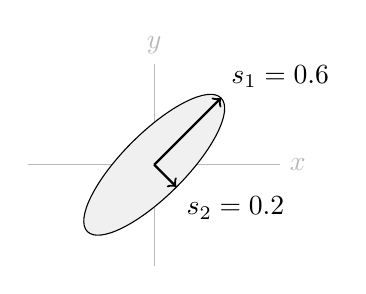
\begin{tikzpicture}[scale=0.8]
\draw[gray!55] (-2,0)--(2,0) node[right] {$x$};
\draw[gray!55] (0,-1.6)--(0,1.6) node[above] {$y$};
\draw[fill=black!6,rotate=45] (0,0) ellipse (1.5 and .5);
\draw[->,thick] (0,0)--(1.06,1.06) node[above right] {$s_1=0.6$};
\draw[->,thick] (0,0)--(.35,-.35) node[below right] {$s_2=0.2$};
\end{tikzpicture}\\
{\small The $1\sigma$ ellipse.
Principal axes have standard deviations 0.6 and 0.2.}
\end{center}
\noindent\textbf{Solution (b).} The function becomes independent of angle at exact isotropy, so the angle derivative vanishes.
Near isotropy, orientation has little effect and can be weakly constrained.
A rotation parameter is not always an observable property.
\Needspace{9\baselineskip}\subsection*{2.2 Gaussian Behavior - Normalization}
Consider one unnormalized 2D kernel $a\exp(-\frac12(x-\mu)^\top\Sigma^{-1}(x-\mu))$ with positive amplitude a > 0.
Double both principal scales while keeping a fixed.
\begin{enumerate}[label=(\alph*),nosep]
\item What happens to its peak value and its integral over the whole plane?
Justify your answer.
\item Does the fourfold integral increase imply fourfold image brightness after projecting and alpha-compositing a 3D splat?
\end{enumerate}
\noindent\textbf{Solution (a).} The peak stays fixed and the integral becomes four times as large.

The principal scales have a direct PCA interpretation.
For samples from one normalized Gaussian $\mathcal N(\mu,\Sigma)$, PCA of the centred samples estimates the eigendecomposition $\Sigma$ = U diag($\lambda$${}_i$) U${}^\top$.
The columns of U are the principal directions, $\lambda$${}_i$ are the variances along them, and the Gaussian scales $s_i=\sqrt{\lambda_i}$ are the corresponding standard deviations.
Finite samples give estimates; eigenvector signs are arbitrary, and repeated eigenvalues do not define unique directions within their eigenspace.

At the mean, the exponent is zero, so the value remains a.
The integral of this unnormalized 2D kernel is a$\cdot$2$\pi$$\cdot$$\sqrt{\det(\Sigma)}$.
Doubling both scales multiplies each covariance eigenvalue by four, and $\sqrt{\det(\Sigma)}$ by four.

A normalized probability density includes the inverse determinant factor and would instead keep unit integral while lowering the peak.
The lab does not include that normalization.
A larger Gaussian therefore changes how much of the domain it covers, even when its peak is unchanged.

This PCA interpretation applies to each Gaussian component.
PCA of a complete probability mixture also reflects variation between component means, so its principal axes can differ from those of the individual Gaussians.
The signed function expansion in this lab is not automatically a probability distribution.
\[
\begin{aligned}\Sigma&=U\operatorname{diag}(\lambda_i)U^\top,\quad s_i=\sqrt{\lambda_i}\\\phi(\mu)&=1,\quad\int a\phi(x)\,dx=a(2\pi)^{d/2}\sqrt{\det\Sigma}\\s_i\mapsto ks_i&\quad\Longrightarrow\quad\text{integral multiplied by }k^d\end{aligned}
\]
\noindent\textbf{Solution (b).} No.
The scalar-field integral is not the image-formation model.
Projection, camera pose, opacity saturation, overlap, and transmittance determine pixel contributions.
The peak opacity of an unnormalized splat stays fixed at its projected mean.
\noindent\href{https://sosekie.github.io/Unibe-CVG-CV-Interactive-Labs/tutorial-09/#dimensions}{Interactive experiment.}
\par\Needspace{18\baselineskip}\section*{3. Fit a 3D scalar function}
\Needspace{9\baselineskip}\subsection*{3.1 Optimization - Gradient Flow}
The 3D model is $\hat{y}$(x) = $a\phi(x;\mu,\Sigma)$, fitted by mean squared error to sampled target values.
Consider the raw gradient at a = 0, with positive scales.
\begin{enumerate}[label=(\alph*),nosep]
\item Which parameters can receive a nonzero loss gradient at that instant?
Justify your answer.
\item Can Adam momentum move a mean when its current raw gradient is zero?
\end{enumerate}
\noindent\textbf{Solution (a).} Amplitude can receive a nonzero gradient, while the mean and covariance gradients are zero.

The derivative with respect to amplitude is $\phi$.
The mean derivative is a$\phi$$\Sigma$${}^{-}$${}^1$(x$-$$\mu$); covariance and scale derivatives also contain a.
At a = 0, the current loss is locally insensitive to geometry, even if prediction error is large.
The amplitude derivative can remain nonzero.

Once amplitude changes, geometry gradients can become nonzero.
Initialization matters in another way: if a narrow kernel lies far from all informative samples, $\phi$ is tiny there and even the amplitude gradient can be weak.
Large residuals alone do not guarantee useful parameter gradients.
\[
\begin{aligned}r_j&=\hat y(x_j)-f(x_j),\quad L=\frac1M\sum_jr_j^2\\\frac{\partial L}{\partial a}&=\frac2M\sum_jr_j\phi_j\\\nabla_\mu L&=\frac2M\sum_jr_j a\phi_j\Sigma^{-1}(x_j-\mu)\end{aligned}
\]
\noindent\textbf{Solution (b).} Yes, if its stored first moment is nonzero from previous updates.
A zero current gradient is not the same as a zero optimizer update.
For the proposed lab experiment, editing an amplitude clears optimizer moments, so the first update isolates the raw-gradient effect.
\Needspace{9\baselineskip}\subsection*{3.2 Approximation - Capacity Vs Optimization}
One Gaussian fits the ring-shaped 3D target poorly after many updates.
Its slices fill the hole or miss much of the ring.
\begin{enumerate}[label=(\alph*),nosep]
\item What can be concluded from the Gaussian model itself, without assuming the optimizer found a global minimum?
Justify your answer.
\item If the displayed volume RMSE is small, could a visually important part of the ring still be poorly fitted?
\end{enumerate}
\noindent\textbf{Solution (a).} One Gaussian cannot represent the target exactly; more optimization may help, but cannot remove this representation mismatch.

For a positive amplitude, every nonempty positive level set of a Gaussian is an ellipsoid enclosing one maximum.
Changing mean, covariance, or amplitude cannot create the ring’s hole.
A nonpositive amplitude cannot reproduce its positive values either.
Exact representation is therefore unavailable with one kernel.

This does not tell us whether the current parameters are optimal within that restricted family.
There may be both approximation error and optimization error.
Several kernels can cover different parts of the ring, but their nonlinear fit can still depend on initialization and the update budget.
\[
a\phi(x)=\tau>0\quad\Longrightarrow\quad(x-\mu)^\top\Sigma^{-1}(x-\mu)=2\log(a/\tau)
\]
\noindent\textbf{Solution (b).} Yes.
Uniform volume MSE averages over many nearly empty samples.
A localized structure can contribute little to the global average while being badly approximated.
Check multiple slices, residual location, and sampling density; consider a region-weighted diagnostic before declaring success.
\noindent\href{https://sosekie.github.io/Unibe-CVG-CV-Interactive-Labs/tutorial-09/#parameters}{Interactive experiment.}
\par\Needspace{18\baselineskip}\section*{4. Project, composite, and expose ambiguity}
\Needspace{9\baselineskip}\subsection*{4.1 Visibility - Photometric Gradients}
At one pixel, a foreground splat has $\alpha_1=0.98$ and a rear splat has $\alpha_2=0.6$.
Hold geometry and opacity fixed while differentiating the pixel colour with respect to the rear RGB.
\begin{enumerate}[label=(\alph*),nosep]
\item What is $\partial$C/$\partial$c${}_2$ for each RGB channel, and what does it imply for fitting?
Justify your answer.
\item Would directly adding the two coloured kernels give the same learning behavior?
\end{enumerate}
\noindent\textbf{Solution (a).} 0.012: foreground transmittance strongly attenuates the rear colour gradient at this pixel.

The foreground leaves T${}_2$ = 1 $-$ 0.98 = 0.02.
The rear contribution is T${}_2$$\alpha$${}_2$c${}_2$, so the per-channel derivative is 0.02 $\times$ 0.6 = 0.012.
A photometric loss gradient contains this factor multiplied by its pixel residual derivative.

A large pixel residual can therefore give little signal to a nearly hidden splat.
With $\alpha$${}_1$ exactly one, this colour gradient would be zero at this pixel.
Other pixels and camera views may expose the rear splat.
Visibility influences which parameters can actually learn from each observation.
\[
\begin{aligned}C&=\alpha_1c_1+(1-\alpha_1)\alpha_2c_2+(1-\alpha_1)(1-\alpha_2)c_{\rm bg}\\\frac{\partial C}{\partial c_2}&=(1-\alpha_1)\alpha_2 I=0.02\cdot0.6\,I=0.012\,I\end{aligned}
\]
\noindent\textbf{Solution (b).} No.
In an additive colour sum, the rear colour derivative would lack the foreground transmittance factor.
Alpha compositing couples visibility and parameter influence; it is not just the scalar basis expansion with RGB outputs.
\Needspace{9\baselineskip}\subsection*{4.2 Multi-View Geometry - Ambiguity}
For an isolated Gaussian and a fixed pinhole camera, multiply its camera-relative mean and all spatial scales by k > 0.
Keep RGB and opacity fixed, and keep it in front of the near plane.
Its locally projected footprint is unchanged.
\begin{enumerate}[label=(\alph*),nosep]
\item Which extra observation generally constrains this depth-scale ambiguity?
Justify your answer.
\item Why can three nearby training views provide less useful depth information than three spread-out views?
\end{enumerate}
\noindent\textbf{Solution (a).} A calibrated image from a different camera centre, with parallax and visibility of the Gaussian.

Scaling camera-relative position preserves x/z and y/z, hence the projected mean.
The pinhole Jacobian scales by 1/k while 3D covariance scales by k${}^2$, preserving the locally projected covariance.
The fixed pixel filter is also unchanged.
The single image cannot distinguish this family of 3D explanations.

Pure rotation about the same optical centre keeps this radial scaling ambiguity.
A translated camera supplies another ray origin and generally makes the two candidate means project differently.
Useful baseline and visibility matter; a second image is not an unconditional guarantee of accurate or unique reconstruction.
\[
\begin{aligned}\mu_{\rm new}&=e+k(\mu-e),\quad\Sigma_{\rm new}=k^2\Sigma,\quad J_{\rm new}=J/k\\J_{\rm new}R^c\Sigma_{\rm new}R^{c\top}J_{\rm new}^\top&=JR^c\Sigma R^{c\top}J^\top\end{aligned}
\]
\noindent\textbf{Solution (b).} With a small translation baseline, viewing rays can be nearly parallel and triangulation becomes sensitive to image error.
A wider baseline can supply stronger depth constraints, while also changing visibility.
More separated views still cannot constrain surfaces they never observe.
\noindent\href{https://sosekie.github.io/Unibe-CVG-CV-Interactive-Labs/tutorial-09/#colour}{Interactive experiment.}
\par\Needspace{18\baselineskip}\section*{5. Recover a scene from images}
\Needspace{9\baselineskip}\subsection*{5.1 Experiment Design - Generalization}
A fit from one selected camera has low training MSE but a much larger reserved-view MSE.
You want to test whether limited view coverage is contributing to the failure.
\begin{enumerate}[label=(\alph*),nosep]
\item Which comparison provides the most relevant controlled evidence?
Justify your answer.
\item If you repeatedly choose budgets and stop times using frame 10, is it still an untouched final test?
\end{enumerate}
\noindent\textbf{Solution (a).} Fit one view and three spread-out views from the same seeds, Gaussian budget, shape mode, and update budget; evaluate both at the reserved pose.

The controlled comparison varies view coverage while holding the initialization and model family fixed.
If the additional views improve reserved-view error, that supports the claim that they supply useful constraints for this fixture.
Compare both training and reserved behavior rather than swapping the metric between runs.

This is evidence, not a universal proof of geometry recovery.
Additional views also change the nonlinear objective, occlusions, and convergence behavior.
Equal update counts here average over each selected set; the multi-view run performs more rendering work per update.
A computation-matched study would control that too.
\[
L_{\rm train}(\theta)=\frac1{|\mathcal V|}\sum_{v\in\mathcal V}\|R(\theta,P_v)-I_v\|^2
\]
\noindent\textbf{Solution (b).} No.
It remains excluded from gradients, but it has become a validation view used for model selection.
An unbiased final performance estimate needs additional untouched views.
This tutorial uses frame 10 as a diagnostic reserved view, not as a benchmark claim.
\Needspace{9\baselineskip}\subsection*{5.2 Density Control - Model Changes}
Consider one isolated coloured splat with opacity o.
Replace it by two coincident splats with identical shape and colour, each with opacity $o^\prime=1-\sqrt{1-o}$.
Let $\phi$ be their shared projected Gaussian value at a pixel.
\begin{enumerate}[label=(\alph*),nosep]
\item Does this opacity adjustment preserve the rendered image everywhere?
Justify your answer.
\item For an additive scalar field, would two coincident copies with amplitudes a/2 preserve the function?
\end{enumerate}
\noindent\textbf{Solution (a).} No: it matches alpha at $\phi$ = 1, but the composited falloff generally differs elsewhere.

At the projected centre, $\phi$ = 1 and 1 $-$ (1$-$o$\prime$)${}^2$ = o by construction.
Away from the centre, the combined alpha is 2o$\prime$$\phi$ $-$ o$\prime$${}^2$$\phi$${}^2$.
That quadratic dependence on $\phi$ is generally different from the original o$\phi$.
The trivial zero-opacity case is unchanged.

Density refinement in the lab also offsets means and may reduce scales, so it changes the forward model further.
More kernels create additional fitting capacity; a heuristic initialization does not preserve the current image or guarantee an immediate decrease in error.
Subsequent optimization must make the new capacity useful.
\[
\begin{aligned}\alpha_{\rm old}&=o\phi,\quad o^\prime=1-\sqrt{1-o}\\\alpha_{\rm pair}&=1-(1-o^\prime\phi)^2=2o^\prime\phi-o^{\prime2}\phi^2\\o=0.75,\ \phi=0.5:&\quad\alpha_{\rm old}=0.375,\quad\alpha_{\rm pair}=0.4375\end{aligned}
\]
\noindent\textbf{Solution (b).} Yes, if their geometry stays identical: (a/2)$\phi$ + (a/2)$\phi$ = a$\phi$ exactly.
This distinction is why arguments about additive basis expansion cannot be transferred unchanged to alpha-composited image fitting.
\noindent\href{https://sosekie.github.io/Unibe-CVG-CV-Interactive-Labs/tutorial-09/#reconstruction}{Interactive experiment.}
\par\Needspace{18\baselineskip}\section*{6. NeRF: a neural field along camera rays}
\Needspace{9\baselineskip}\subsection*{6.1 Volume Rendering - Optical Thickness}
A ray crosses a homogeneous slab of length $L=1$ with density $\sigma=2$ and constant RGB.
You approximate it with N equal intervals of length $\delta=L/N$, using $\alpha_i=1-\exp(-\sigma\delta)$.
\begin{enumerate}[label=(\alph*),nosep]
\item What happens to total transmittance if you change N from 10 to 100?
Justify your answer.
\item If a thin high-density feature lies entirely between the sample points, does a low sampled density prove the ray is empty?
\end{enumerate}
\noindent\textbf{Solution (a).} It stays exp($-$2); each smaller interval has proportionally less optical thickness.

Each interval transmits exp($-$$\sigma$L/N).
Multiplying N such factors gives exp($-$$\sigma$L), independent of N.
Here $T_{\mathrm{end}}$ = exp($-$2), approximately 0.1353.
With constant colour, the slab contribution is (1$-$exp($-$2))c, plus the remaining background.

Density has units of inverse distance; alpha is dimensionless and depends on interval length.
Holding alpha fixed while increasing N would change the modeled optical thickness.
For a spatially varying field, additional samples can improve the numerical integral when they resolve its variation; the homogeneous example is exactly integrated by this rule.
\[
\begin{aligned}\delta&=L/N,\quad\alpha_i=1-e^{-\sigma\delta}\\T_{\rm end}&=\prod_{i=1}^N e^{-\sigma L/N}=e^{-\sigma L}=e^{-2}\approx0.1353\end{aligned}
\]
\noindent\textbf{Solution (b).} No.
Midpoint samples can miss a thin feature.
Increasing or redistributing samples addresses integration error of the current field.
It does not by itself add observations, learn the missing structure, or guarantee a correct field.
Distinguish field approximation from quadrature error.
\Needspace{9\baselineskip}\subsection*{6.2 Neural Fields - Multi-View Consistency}
In a classical NeRF-style model, density is $\sigma_\theta(x)$, while RGB is $c_\theta(x,d)$.
A proposed variant also lets density depend freely on viewing direction: $\sigma_\theta(x,d)$.
\begin{enumerate}[label=(\alph*),nosep]
\item Why is position-only density a useful constraint for reconstructing a static scene?
Justify your answer.
\item Is increasing the number of samples per ray the NeRF equivalent of adding more Gaussian primitives?
\end{enumerate}
\noindent\textbf{Solution (a).} It makes different cameras query the same spatial extinction field, while allowing directional appearance in the RGB branch.

A static spatial density field should supply consistent extinction at the same location across views.
Restricting density to position encourages the cameras to explain images using shared structure.
Colour can still depend on direction, allowing view-related appearance changes without directly changing the density at that position.

The network weights are adjusted through a differentiable pixel loss.
The network is not given a target density at every sample.
Direction-dependent density could make independent per-view explanations easier, while position-only density still does not remove all image-based ambiguities.
Coverage, initialization, architecture, and optimization continue to matter.
\[
\sigma=\sigma_\theta(x),\quad c=c_\theta(x,d),\qquad\theta\leftarrow\theta-\eta\nabla_\theta L_{\rm pixels}
\]
\noindent\textbf{Solution (b).} No.
More ray samples change where and how accurately a fixed field is evaluated; network parameter count stays fixed.
Adding Gaussians changes the explicit scene parameterization.
Sampling also changes the numerical gradients used during subsequent fitting, so it can affect learning even though it does not increase neural-field capacity.
\noindent\href{https://sosekie.github.io/Unibe-CVG-CV-Interactive-Labs/tutorial-09/#nerf}{Interactive experiment.}
\par\Needspace{18\baselineskip}\section*{7. Transfer to the real captured Garden}
\Needspace{9\baselineskip}\subsection*{7.1 Appearance - Representation Choice}
Suppose a glossy leaf changes brightness with viewing direction in the captured photographs, but a reconstruction represents each Gaussian with one fixed RGB value.
Even with good spatial coverage, a highlight appears painted onto the surface.
\begin{enumerate}[label=(\alph*),nosep]
\item Which model change directly addresses this missing behavior?
Justify your answer.
\item Could a low photometric error prove that positions and covariances are correct when colour is very flexible?
\end{enumerate}
\noindent\textbf{Solution (a).} Let each Gaussian’s emitted colour depend on viewing direction, for example through spherical harmonics.

The spatial Gaussian specifies local support; the appearance model specifies colour.
A fixed RGB value cannot directly express a view-dependent highlight.
Direction-dependent colour coefficients add that degree of freedom.
Full 3DGS uses spherical harmonics for this purpose; the compact Garden viewer used here displays RGB appearance.

Additional spatial splats may partly compensate for an inadequate appearance model, but that can entangle geometry and colour rather than model the directional effect directly.
Higher output resolution changes sampling, not the trained appearance parameters.
A richer appearance model also needs observations that constrain it.
\[
c_i(d)=\sum_{\ell,m}\beta_{i,\ell m}Y_{\ell m}(d)
\]
\noindent\textbf{Solution (b).} No.
Geometry and appearance can compensate for each other under finite observations.
Evaluate new viewing directions and, when geometry matters, use independent geometric evidence.
Directional colour increases expressiveness; it is not a uniqueness guarantee.
\Needspace{9\baselineskip}\subsection*{7.2 Transfer - Rendering Vs Geometry}
The garden looks sharp from several viewpoints.
A colleague wants to treat the visible Gaussian ellipsoids as a reliable surface model for collision detection.
\begin{enumerate}[label=(\alph*),nosep]
\item What does the rendering evidence justify?
Justify your answer.
\item If rendering at twice the resolution reveals smaller floaters, has the underlying geometry become worse?
\end{enumerate}
\noindent\textbf{Solution (a).} It supports appearance quality from those views; reliable collision geometry needs additional geometric validation and a defined surface representation.

A photometric objective constrains rendered rays.
It does not directly supervise a watertight boundary, distances, or normals.
Gaussian ellipsoids describe spatial kernels; a 1$\sigma$ contour is a visualization convention, not a measured surface.
Overlapping, partially transparent primitives can explain images without defining unique collision geometry.

For a geometry-dependent application, define how a surface is obtained and validate it against independent depth, geometry, or task-relevant measurements, including previously occluded regions.
An accurate renderer can be valuable for novel-view synthesis while remaining insufficient evidence for a different task.
\[
\text{Low image error on observed rays}\quad\not\Rightarrow\quad\text{low surface-distance error}
\]
\noindent\textbf{Solution (b).} No.
Changing output resolution can expose existing artifacts without changing the stored model.
Distinguish representation quality, observation coverage, and display sampling when explaining what you see.
\noindent\href{https://sosekie.github.io/Unibe-CVG-CV-Interactive-Labs/tutorial-09/#highres}{Interactive experiment.}
\end{document}
